\section{HTML5 Web Workers} \label{chapter_webworkers}

For efficient machine utilization and speedups, HPC applications must make use of all available CPU cores by designing the application with respect to intra-node processing capabilities. Traditionally, this is realized by using multiple threads in a process. While each thread may allocate its own memory, currently common shared memory systems allow direct access of shared memory between all threads. 

Until the release of HTML5, an HTML document's JavaScript script was always executed in a single thread. To allow threaded execution, HTML5 specified Web Workers. The main thread can spawn Web Workers and assign a script file to them, as seen in listing \ref{ww_main}. This script file can contain arbitrary code to be executed in its own thread, asynchronously from the main thread. See listing \ref{ww_script}. One constraint for Web Workers is that they cannot access and manipulate the HTML document's DOM; only the main thread is able to do that.

\lstset{caption={Main thread spawns Web Worker},label=ww_main}
\begin{lstlisting}[frame=single,basicstyle=\footnotesize]
var worker = new Worker("worker_script.js");

worker.addEventListener("message", function(e) {
  console.log(e.data);
}, false);

worker.postMessage("Hello!");
\end{lstlisting}

\lstset{caption={Web Worker script},label=ww_script}
\begin{lstlisting}[frame=single,basicstyle=\footnotesize]
self.addEventListener("message", function(e) {
  // Async computations go here
  self.postMessage(e.data);
}, false);
\end{lstlisting}


\subsection{Message Passing}

Another constraint for Web Workers is that shared memory is not possible. Memory allocated in the main thread or in a Web Worker is never accessible by others. Communication is based on message passing. This is done by using the postMessage function. One has to differentiate between two use cases of this function.

By simply handing an object to postMessage, a structured cloning on this object is performed to create a copy. This copy is made available to the Web Worker; direct access to the original is not possible. Structured cloning is the way to systematically copy JSON objects, which can be hierarchically nested. Copying such data structeres is detrimental for achieved bandwidth. On the machine used for this work, postMessage structured cloning of a simple array caps at around 1 GB/s, as seen in figure \ref{fig:ww_bw}. As arrays are continously stored in memory, this actually represents the upper limit. Compared to traditional shared memory accesses, this is hardly acceptable for HPC applications.

Additional issues may arise from sending messages of several MBs in size too fast. The garbage collector might potentially not be fast enough in freeing unused copied messages. Results might be huge or spiked memory consumption, or even an application crash if memory is exhausted.

\begin{figure}[htp]
  \begin{center}
    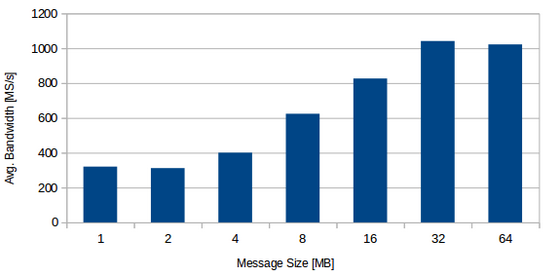
\includegraphics[width=0.9\columnwidth]{resources/ww_bw.png}
  \end{center}
  \caption{postMessage structured cloning bandwidth of an array}
  \label{fig:ww_bw}
\end{figure}

Alternatively, transferable objects can be send via postMessage. Transferable objects are simple data structures like arrays, which need no structured cloning. The syntax used is shown in listing \ref{ww_trans}. It is important to note that sent data switch contexts. After the call to postMessage, the sender has no longer access to the data; the variable evaluates to null. Only the receiver has access now. This is realized internally by simple pointer exchanges, making bandwidth measurements obsolete. The latency for this operation on the machine used for this work is 53us. HPC applications should structure their Web Workers communication using this approach.

\lstset{caption={Sending a transferable object array},label=ww_trans}
\begin{lstlisting}[frame=single,basicstyle=\footnotesize]
var array = new ArrayBuffer(1024); // 1kB
worker.postMessage(array.buffer, [array.buffer]);
\end{lstlisting}


\subsection{Compatibility}

Web Workers are basically supported in all modern web browser. Unfortunately, sending transferable objects via postMessage is not part of the HTML5 specification. Currently, Internet Explorer does not support transferable objects via postMessage.
